\documentclass[11pt,a4paper]{article}
\usepackage[utf8]{inputenc}
\usepackage[T1]{fontenc}
\usepackage[spanish,provide=*]{babel}
\usepackage{lmodern}
\usepackage{amsmath,amssymb,amsthm}
\usepackage[margin=2.54cm]{geometry}
\usepackage{graphicx}
\usepackage{tikz}
\usepackage{pgfplots}
\pgfplotsset{compat=1.18}
\usepackage[hidelinks]{hyperref}

\newtheorem{teorema}{Teorema}[section]
\newtheorem{proposicion}[teorema]{Proposición}
\theoremstyle{definition}
\newtheorem{definicion}[teorema]{Definición}
\newtheorem{ejemplo}[teorema]{Ejemplo}

\title{Plantilla de notas matemáticas}
\author{}
\date{}

\begin{document}
\maketitle

\section{Comprobación del entorno}
Esta plantilla verifica la compilación de texto en español, expresiones
matemáticas y gráficos vectoriales. Sustituir su contenido al preparar un apunte.

\begin{definicion}
Para $n\in\mathbb{N}$, un vector columna $\boldsymbol{x}\in\mathbb{R}^{n}$
se escribe como
\[
\boldsymbol{x}=\begin{pmatrix}x_1\\x_2\\\vdots\\x_n\end{pmatrix},
\qquad x_i\in\mathbb{R}\quad (i=1,\ldots,n).
\]
\end{definicion}

\begin{center}
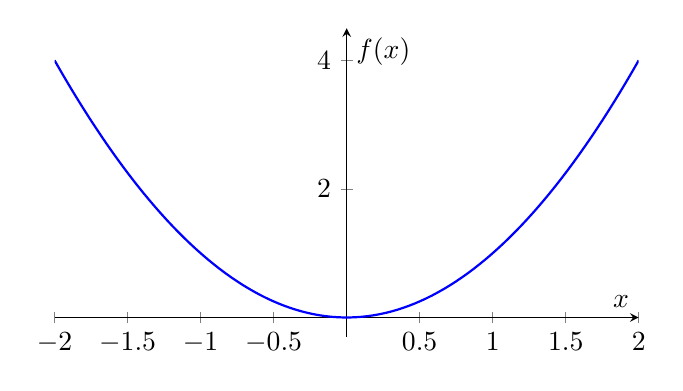
\begin{tikzpicture}
\begin{axis}[width=9cm,height=5.5cm,axis lines=middle,
  xlabel={$x$},ylabel={$f(x)$},xmin=-2,xmax=2,ymin=-0.3,ymax=4.5,
  domain=-2:2,samples=100]
\addplot[blue,thick] {x^2};
\end{axis}
\end{tikzpicture}
\end{center}

\end{document}
